% Options for packages loaded elsewhere
\PassOptionsToPackage{unicode}{hyperref}
\PassOptionsToPackage{hyphens}{url}
\PassOptionsToPackage{dvipsnames,svgnames,x11names}{xcolor}
%
\documentclass[
  letterpaper,
  DIV=11,
  numbers=noendperiod,
  oneside]{scrartcl}

\usepackage{amsmath,amssymb}
\usepackage{iftex}
\ifPDFTeX
  \usepackage[T1]{fontenc}
  \usepackage[utf8]{inputenc}
  \usepackage{textcomp} % provide euro and other symbols
\else % if luatex or xetex
  \usepackage{unicode-math}
  \defaultfontfeatures{Scale=MatchLowercase}
  \defaultfontfeatures[\rmfamily]{Ligatures=TeX,Scale=1}
\fi
\usepackage{lmodern}
\ifPDFTeX\else  
    % xetex/luatex font selection
\fi
% Use upquote if available, for straight quotes in verbatim environments
\IfFileExists{upquote.sty}{\usepackage{upquote}}{}
\IfFileExists{microtype.sty}{% use microtype if available
  \usepackage[]{microtype}
  \UseMicrotypeSet[protrusion]{basicmath} % disable protrusion for tt fonts
}{}
\makeatletter
\@ifundefined{KOMAClassName}{% if non-KOMA class
  \IfFileExists{parskip.sty}{%
    \usepackage{parskip}
  }{% else
    \setlength{\parindent}{0pt}
    \setlength{\parskip}{6pt plus 2pt minus 1pt}}
}{% if KOMA class
  \KOMAoptions{parskip=half}}
\makeatother
\usepackage{xcolor}
\usepackage[left=1in,marginparwidth=2.0666666666667in,textwidth=4.1333333333333in,marginparsep=0.3in]{geometry}
\setlength{\emergencystretch}{3em} % prevent overfull lines
\setcounter{secnumdepth}{-\maxdimen} % remove section numbering
% Make \paragraph and \subparagraph free-standing
\makeatletter
\ifx\paragraph\undefined\else
  \let\oldparagraph\paragraph
  \renewcommand{\paragraph}{
    \@ifstar
      \xxxParagraphStar
      \xxxParagraphNoStar
  }
  \newcommand{\xxxParagraphStar}[1]{\oldparagraph*{#1}\mbox{}}
  \newcommand{\xxxParagraphNoStar}[1]{\oldparagraph{#1}\mbox{}}
\fi
\ifx\subparagraph\undefined\else
  \let\oldsubparagraph\subparagraph
  \renewcommand{\subparagraph}{
    \@ifstar
      \xxxSubParagraphStar
      \xxxSubParagraphNoStar
  }
  \newcommand{\xxxSubParagraphStar}[1]{\oldsubparagraph*{#1}\mbox{}}
  \newcommand{\xxxSubParagraphNoStar}[1]{\oldsubparagraph{#1}\mbox{}}
\fi
\makeatother


\providecommand{\tightlist}{%
  \setlength{\itemsep}{0pt}\setlength{\parskip}{0pt}}\usepackage{longtable,booktabs,array}
\usepackage{calc} % for calculating minipage widths
% Correct order of tables after \paragraph or \subparagraph
\usepackage{etoolbox}
\makeatletter
\patchcmd\longtable{\par}{\if@noskipsec\mbox{}\fi\par}{}{}
\makeatother
% Allow footnotes in longtable head/foot
\IfFileExists{footnotehyper.sty}{\usepackage{footnotehyper}}{\usepackage{footnote}}
\makesavenoteenv{longtable}
\usepackage{graphicx}
\makeatletter
\def\maxwidth{\ifdim\Gin@nat@width>\linewidth\linewidth\else\Gin@nat@width\fi}
\def\maxheight{\ifdim\Gin@nat@height>\textheight\textheight\else\Gin@nat@height\fi}
\makeatother
% Scale images if necessary, so that they will not overflow the page
% margins by default, and it is still possible to overwrite the defaults
% using explicit options in \includegraphics[width, height, ...]{}
\setkeys{Gin}{width=\maxwidth,height=\maxheight,keepaspectratio}
% Set default figure placement to htbp
\makeatletter
\def\fps@figure{htbp}
\makeatother
% definitions for citeproc citations
\NewDocumentCommand\citeproctext{}{}
\NewDocumentCommand\citeproc{mm}{%
  \begingroup\def\citeproctext{#2}\cite{#1}\endgroup}
\makeatletter
 % allow citations to break across lines
 \let\@cite@ofmt\@firstofone
 % avoid brackets around text for \cite:
 \def\@biblabel#1{}
 \def\@cite#1#2{{#1\if@tempswa , #2\fi}}
\makeatother
\newlength{\cslhangindent}
\setlength{\cslhangindent}{1.5em}
\newlength{\csllabelwidth}
\setlength{\csllabelwidth}{3em}
\newenvironment{CSLReferences}[2] % #1 hanging-indent, #2 entry-spacing
 {\begin{list}{}{%
  \setlength{\itemindent}{0pt}
  \setlength{\leftmargin}{0pt}
  \setlength{\parsep}{0pt}
  % turn on hanging indent if param 1 is 1
  \ifodd #1
   \setlength{\leftmargin}{\cslhangindent}
   \setlength{\itemindent}{-1\cslhangindent}
  \fi
  % set entry spacing
  \setlength{\itemsep}{#2\baselineskip}}}
 {\end{list}}
\usepackage{calc}
\newcommand{\CSLBlock}[1]{\hfill\break\parbox[t]{\linewidth}{\strut\ignorespaces#1\strut}}
\newcommand{\CSLLeftMargin}[1]{\parbox[t]{\csllabelwidth}{\strut#1\strut}}
\newcommand{\CSLRightInline}[1]{\parbox[t]{\linewidth - \csllabelwidth}{\strut#1\strut}}
\newcommand{\CSLIndent}[1]{\hspace{\cslhangindent}#1}

% load packages
\usepackage{geometry}
\usepackage{xcolor}
\usepackage{eso-pic}
\usepackage{fancyhdr}
\usepackage{sectsty}
\usepackage{fontspec}
\usepackage{titlesec}

%% Set page size with a wider right margin
\geometry{a4paper, total={170mm,257mm}, left=20mm, top=20mm, bottom=20mm, right=50mm}

%% Let's define some colours
\definecolor{light}{HTML}{E6E6FA}
\definecolor{highlight}{HTML}{800080}
\definecolor{dark}{HTML}{330033}

%% Let's add the border on the right hand side 
\AddToShipoutPicture{% 
    \AtPageLowerLeft{% 
        \put(\LenToUnit{\dimexpr\paperwidth-3cm},0){% 
            \color{light}\rule{3cm}{\LenToUnit\paperheight}%
          }%
     }%
     % logo
    \AtPageLowerLeft{% start the bar at the bottom right of the page
        \put(\LenToUnit{\dimexpr\paperwidth-2.25cm},27.2cm){% move it to the top right
            \color{light}
\includegraphics[width=1.5cm]{_extensions/nrennie/PrettyPDF/logo.png}
          }%
     }%
}

%% Style the page number
\fancypagestyle{mystyle}{
  \fancyhf{}
  \renewcommand\headrulewidth{0pt}
  \fancyfoot[R]{\thepage}
  \fancyfootoffset{3.5cm}
}
\setlength{\footskip}{20pt}

%% style the chapter/section fonts
\chapterfont{\color{dark}\fontsize{20}{16.8}\selectfont}
\sectionfont{\color{dark}\fontsize{20}{16.8}\selectfont}
\subsectionfont{\color{dark}\fontsize{14}{16.8}\selectfont}
\titleformat{\subsection}
  {\sffamily\Large\bfseries}{\thesection}{1em}{}[{\titlerule[0.8pt]}]
  
% left align title
\makeatletter
\renewcommand{\maketitle}{\bgroup\setlength{\parindent}{0pt}
\begin{flushleft}
  {\sffamily\huge\textbf{\MakeUppercase{\@title}}} \vspace{0.3cm} \newline
  {\Large {\@subtitle}} \newline
  \@author
\end{flushleft}\egroup
}
\makeatother

%% Use some custom fonts
\setsansfont{Ubuntu}[
    Path=_extensions/nrennie/PrettyPDF/Ubuntu/,
    Scale=0.9,
    Extension = .ttf,
    UprightFont=*-Regular,
    BoldFont=*-Bold,
    ItalicFont=*-Italic,
    ]

\setmainfont{Ubuntu}[
    Path=_extensions/nrennie/PrettyPDF/Ubuntu/,
    Scale=0.9,
    Extension = .ttf,
    UprightFont=*-Regular,
    BoldFont=*-Bold,
    ItalicFont=*-Italic,
    ]
\KOMAoption{captions}{tableheading}
\makeatletter
\@ifpackageloaded{caption}{}{\usepackage{caption}}
\AtBeginDocument{%
\ifdefined\contentsname
  \renewcommand*\contentsname{Table of contents}
\else
  \newcommand\contentsname{Table of contents}
\fi
\ifdefined\listfigurename
  \renewcommand*\listfigurename{List of Figures}
\else
  \newcommand\listfigurename{List of Figures}
\fi
\ifdefined\listtablename
  \renewcommand*\listtablename{List of Tables}
\else
  \newcommand\listtablename{List of Tables}
\fi
\ifdefined\figurename
  \renewcommand*\figurename{Figure}
\else
  \newcommand\figurename{Figure}
\fi
\ifdefined\tablename
  \renewcommand*\tablename{Table}
\else
  \newcommand\tablename{Table}
\fi
}
\@ifpackageloaded{float}{}{\usepackage{float}}
\floatstyle{ruled}
\@ifundefined{c@chapter}{\newfloat{codelisting}{h}{lop}}{\newfloat{codelisting}{h}{lop}[chapter]}
\floatname{codelisting}{Listing}
\newcommand*\listoflistings{\listof{codelisting}{List of Listings}}
\makeatother
\makeatletter
\makeatother
\makeatletter
\@ifpackageloaded{caption}{}{\usepackage{caption}}
\@ifpackageloaded{subcaption}{}{\usepackage{subcaption}}
\makeatother
\makeatletter
\@ifpackageloaded{tcolorbox}{}{\usepackage[skins,breakable]{tcolorbox}}
\makeatother
\makeatletter
\@ifundefined{shadecolor}{\definecolor{shadecolor}{rgb}{.97, .97, .97}}{}
\makeatother
\makeatletter
\@ifundefined{codebgcolor}{\definecolor{codebgcolor}{named}{light}}{}
\makeatother
\makeatletter
\ifdefined\Shaded\renewenvironment{Shaded}{\begin{tcolorbox}[breakable, boxrule=0pt, colback={codebgcolor}, frame hidden, enhanced, sharp corners]}{\end{tcolorbox}}\fi
\makeatother
\makeatletter
\@ifpackageloaded{sidenotes}{}{\usepackage{sidenotes}}
\@ifpackageloaded{marginnote}{}{\usepackage{marginnote}}
\makeatother
\makeatletter
\@ifpackageloaded{fontawesome5}{}{\usepackage{fontawesome5}}
\makeatother

\ifLuaTeX
  \usepackage{selnolig}  % disable illegal ligatures
\fi
\usepackage{bookmark}

\IfFileExists{xurl.sty}{\usepackage{xurl}}{} % add URL line breaks if available
\urlstyle{same} % disable monospaced font for URLs
\hypersetup{
  colorlinks=true,
  linkcolor={highlight},
  filecolor={Maroon},
  citecolor={Blue},
  urlcolor={highlight},
  pdfcreator={LaTeX via pandoc}}


\author{}
\date{}

\begin{document}

\pagestyle{mystyle}


\section{Nocturnal Cinema}\label{nocturnal-cinema}

\subsection{Film Noir, Jazz, and the French New
Wave}\label{film-noir-jazz-and-the-french-new-wave}

\marginnote{\begin{footnotesize}

\href{https://mroberts.emerson.build/}{Martin Roberts}~\\
\href{https://emerson.edu/academics/academic-departments/visual-media-arts}{Department
of Visual \& Media Arts}\\
\href{https://emerson.edu}{Emerson College}\\
\href{https://theurbannight.files.wordpress.com/2022/03/book-of-abstracts.pdf}{Media
\& The Night Conference}\\
McGill University\\
18-19 March 2022\\
\href{mailto:martin_roberts@emerson.edu}{\faIcon{envelope}} \textbar{}
\href{https://merveilles.town/@mroberts_vma}{\faIcon{mastodon}}
\textbar{} \href{https://github.com/mroberts1/}{\faIcon{github}}
\textbar{} \href{https://facebook.com/mr05301}{\faIcon{facebook}}
\textbar{} \href{https://twitter.com/dokoissho}{\faIcon{twitter}}

\end{footnotesize}}

\begin{figure}[H]

{\centering 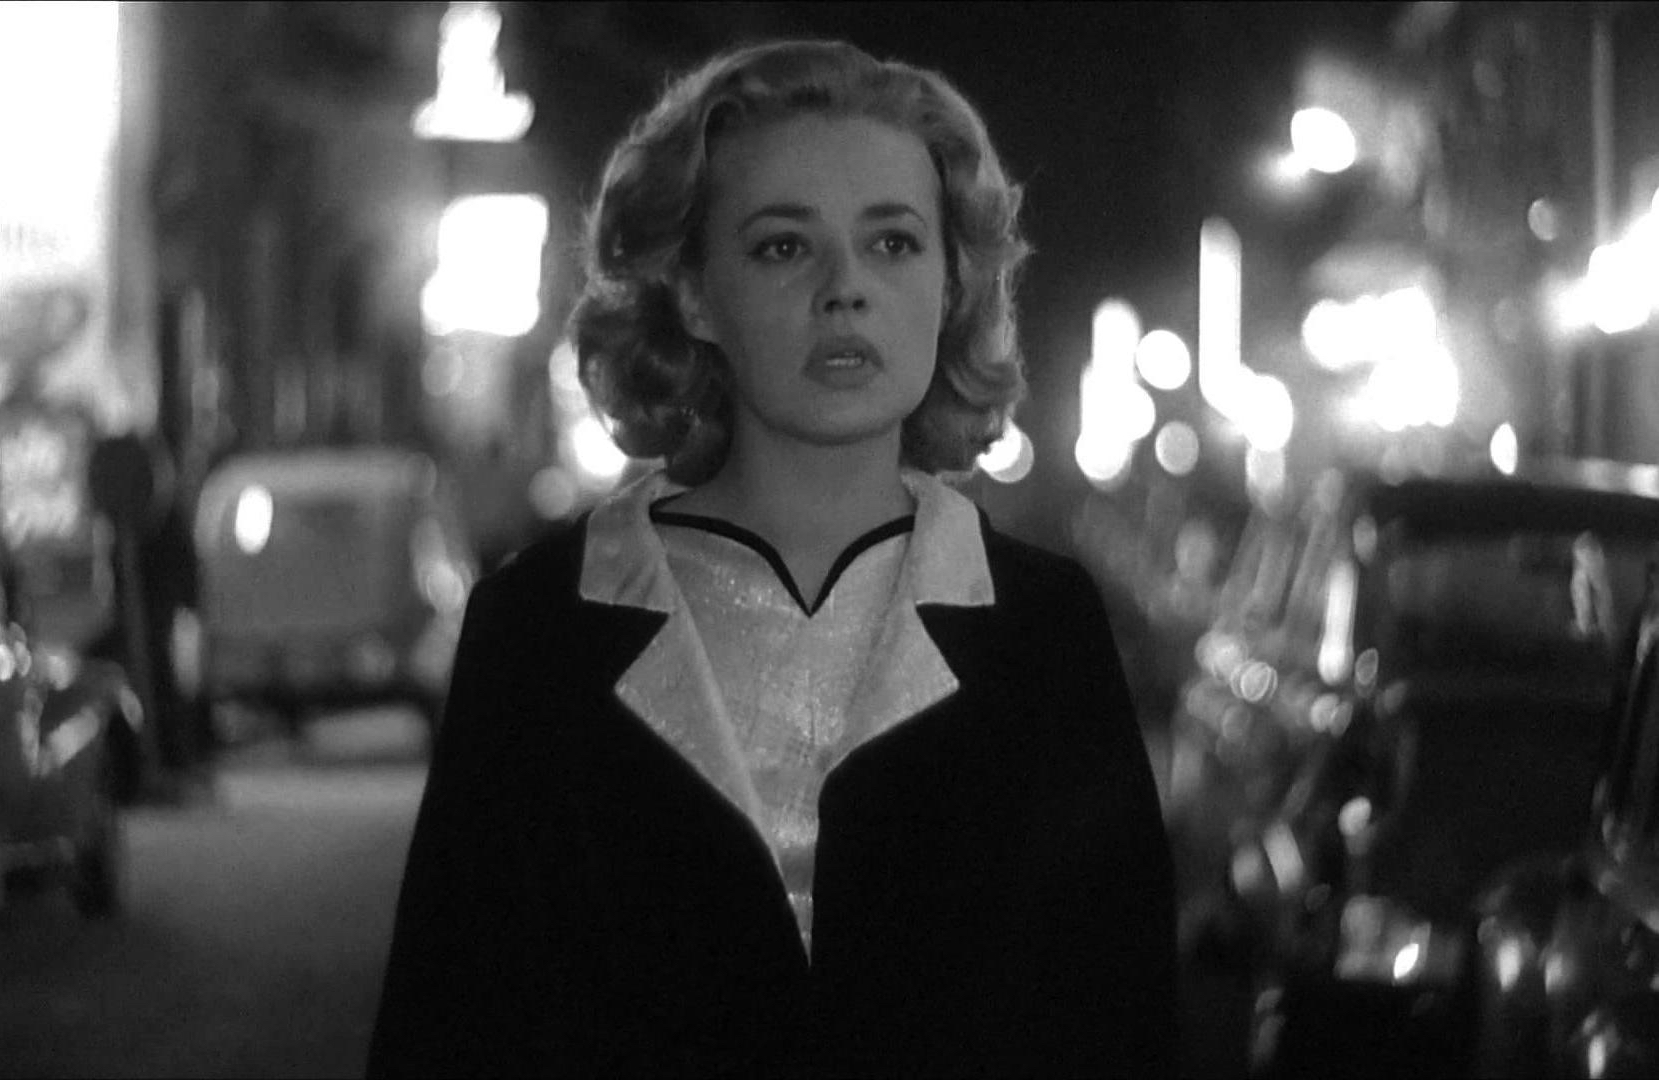
\includegraphics{img/ascenseur.jpg}

}

\caption{\emph{Ascenseur pour l'échafaud} (Louis Malle, 1958)}

\end{figure}%

\begin{center}\rule{0.5\linewidth}{0.5pt}\end{center}

\begin{quote}
Le cinéma s'est approprié la nuit pour la réinventer et, depuis, notre
perception n'est plus la même. {\marginnote{\begin{footnotesize}Cinema
appropriated night in order to reinvent it, and our perception of it has
never been the same since. It's hard to look at Shanghai or New York
without thinking about \emph{Blade Runner}. The pleasures of nocturnal
\emph{flâneurs}; the night of crooks, dealers, and down-and-outs; the
night of dreams or the everyday night of workers\ldots{} By its magic,
the seventh art has taken hold of the night in order to turn it into a
character in its own right. {[}All translations mine.
{]}\end{footnotesize}}}Difficile de contempler Shanghai ou New York sans
penser à \emph{Blade Runner}. Plaisirs de noctambules, nuit des truands,
des dealers et des paumés, nuit de rêve ou quotidien des travailleurs
nocturnes\ldots{} , par sa magie, le septième art s'est emparé de la
nuit pour en faire un personnage à part entière.

-- Luc Gwiazdzinski (2016: 63).
\end{quote}

\begin{quote}
{[}L{]}a nuit suggère, elle ne montre
pas.{\marginnote{\begin{footnotesize}The night doesn't show, it
suggests. It disturbs and surprises us by its strangeness; it triggers
impulses in us that, during the day, are dominated by reason. . . . I
loved the wonders of the night that light forced to manifest themselves;
absolute night does not exist.\end{footnotesize}}} La nuit nous trouble
et nous surprend par son étrangeté; elle libère des forces en nous qui,
le jour, sont dominées par la raison. . . . J'aimais les prodiges de la
nuit que la lumière contraignait à se manifester; il n'existe pas une
nuit absolue.

-- Brassaï, feuillet inédit, archives Gilberte Brassaï, no date
(Exposition «Brassaï», Centre Georges Pompidou, 2000).
\end{quote}

\begin{quote}
Black and white are, for me, cinema's most beautiful colours.

-- Rainer Werner Fassbinder (cited in Misek 2010: 83).
\end{quote}

\begin{center}\rule{0.5\linewidth}{0.5pt}\end{center}

\subsubsection{Avant-Propos / Preamble}\label{avant-propos-preamble}

I'd like to start with a brief disclaimer about what I am trying to do
in this paper, and---just as importantly---what I am \emph{not} trying
to do. As many people here will no doubt be already aware, there has
existed for some time now a voluminous and highly specialized body of
literature on the genre of \emph{film noir}, and on the postwar movement
in French film known as the \emph{nouvelle vague} or New Wave. While I
have no pretensions to adding to that literature, its existence does not
mean that everything there is to say on these subjects has already been
said. Maybe I've just been watching too many heist movies lately, but
what I am interested in doing is to try---under cover of darkness,
obviously---to break open the constrictive generic and auteurist vaults
in which cinema has been locked away for decades by introducing a
different paradigm that I call \emph{nocturnal cinema}. While the night
has figured prominently in cinema from its earliest origins, by
nocturnal cinema I am referring to a more specific corpus of films in
which night is not just a temporal backdrop for narrative realism but is
foregrounded as an aesthetic, thematic, stylistic, and symbolic element
in the films in question. The paradigm of nocturnal cinema, I want to
suggest, opens up the possibility of conceptualizing alternative
histories of cinema that treat it not as a discrete object of study but
position it within a broader cultural spectrum of media and artistic
practices. As such, it may serve as a prototype for other new ways of
thinking about the history of cinema.

With that said, let us begin, as one must, with Melville.

\subsubsection{Pigalle}\label{pigalle}

This sequence from \emph{Bob le flambeur} provides a succinct example of
a particular kind of cinematic cultural mythology that was already in
place when Melville's film was released in 1956: a set of associations
involving criminal activity, music, and the urban night, originating in
the cinematic appropriation of popular crime fiction, that in the late
1940s came to be known as \emph{film noir}. The emergence of this
mythology in the late-1930s films of Marcel Carné, and over subsequent
decades in the films of Jules Dassin, Jacques Becker, Jean-Pierre
Melville, Louis Malle, and Édouard Molinaro, followed by the
\emph{nouvelle vague} films of Godard, Truffaut, Chabrol, and others, is
the subject both of the present paper and a related project I am
currently working on, a cinematic compilation album titled
\emph{Ciné-Jazz}.

\marginnote{\begin{footnotesize}

\end{footnotesize}}

For reasons of time, I will limit myself here to the work of Édouard
Molinaro, which has been overshadowed by the better-known examples of
Louis Malle's celebrated collaboration with Miles Davis on
\emph{Ascenseur pour l'échafaud} (1958), Godard's \emph{À bout de
souffle} (1960), and others. The series of films released by Molinaro in
the late 1950s that includes \emph{Le dos au mur} (1958), \emph{Des
femmes disparaissent} (1959, and \emph{Un témoin dans la ville} (1959),
embody the cinematic chronotope of urban crime, jazz, and the night.
Collectively, they provide a case study in a larger genre that I would
like to call \emph{nocturnal cinema}. I want to explore here some of the
key characteristics of this nocturnal cinema, as manifested in French
\emph{film noir} and its legacy in the \emph{nouvelle vague} or New
Wave.

\subsubsection{Nuits Monochromes}\label{nuits-monochromes}

As a quintessentially nocturnal experience of urban modernity, cinema is
almost organically related to the night; as Luc Gwiazdzinski has
observed,

\begin{quote}
Du noir de la pellicule à l'obscurité de ses salles, le cinéma
entretient un rapport quasi physique avec la
nuit.{\marginnote{\begin{footnotesize}From the blackness of celluloid to
the darkness of movie theaters, cinema has an almost physical
relationship to night. Nothing seems able to escape the hold of night.
It's often more difficult to appreciate a film that takes place in
daylight: even projected in a dark room, the film loses its intensity
after we leave, the mystery and magic fade too
quickly.\end{footnotesize}}} Rien ne semble pouvoir échapper à l'emprise
de la nuit. Il est souvent plus difficile d'apprécier un film en
journée: même projeté dans une salle obscure, le film perd de son
intensité et à la sortie, le mystère et la magie s'estompent trop vite
(2016: 62).
\end{quote}

But if the urban experience of watching movies has historically taken
place in nocturnal darkness, the nocturnal city itself has been a
subject of predilection for cinema since its inception; consider, for
example, the early movies of Edison cameraman Edwin Porter, of the
dazzling lights of the \href{https://youtu.be/Q5m6joTlnqA}{Pan-American
exhibition} or \href{https://www.youtube.com/watch?v=NqDtG3dcxPs}{Coney
Island} at night. There is a residual sense of wonder, what David Nye
calls the electrical sublime, in the nocturnal cityscapes of Molinaro
and other filmmakers of his time, the ``magie'' of the night alluded to
by Gwiadzdinski; but I would argue that by the 1950s this had been
displaced by a deep ambivalence about the night as a space both of
temptation, of opportunity for financial and erotic gain unavailable in
the mundane light of day, but also a space of danger, or more accurately
dangerous liaisons that lead to the downfall of those who embrace them.

The urban night is also the privileged chronotope of \emph{film noir},
whether in its American, French, or British incarnations, and that
night, with its deserted streets, its neon-drenched demi-monde of bars
and cabarets, is the pre-eminent setting for shady goings-on of all
kinds, from jewel heists to prostitution to drug deals to the disposal
of bodies. But while the night provides the backdrop to such activities
in \emph{film noir}, from Fritz Lang's \emph{The Woman in the Window}
(1944) to Jules Dassin's \emph{Night and the City} (1950), it takes on a
particularly luminous resonance in the French cinema of the 1950s, from
the films of Melville, as we have seen, to Louis Malle's \emph{Ascenseur
pour l'échafaud} (1958), with its famous sequence of Jean Moreau
prowling the Parisian streets in search of her missing lover,
accompanied by Miles Davis's muted trumpet.

Although less common in \emph{film noir} than is often assumed, jazz
soundtracks are a key component of nocturnal cinema, in part because of
the music's own associations with nocturnal entertainment. Not only
Miles Davis, but many other American jazz musicians performed in Paris
in the late 1950s, including Donald Byrd, Thelonious Monk, and Art
Blakey, in addition to musicians already based there such as René
Urtreger, Franco-American Barney Wilen, and Algerian-born Martial Solal.
Various permutations of these musicians were tapped to write soundtracks
for French films: Art Blakey's Jazz Messengers for Molinaro's \emph{Des
Femmes disparaissent} and Roger Vadim's \emph{Les Liaisons dangereuses};
Monk also for \emph{Les Liaisons dangereuses}; Barney Wilen and Kenny
Dorham for \emph{Un témoin dans la ville}; Martial Solal for Godard's
\emph{À bout de souffle}.

\marginnote{\begin{footnotesize}

\end{footnotesize}}

It is, however, in the nocturnal cinema of Édouard Molinaro that the
aesthetic resonance of the urban night reaches its fullest expression;
so tangible does its presence become that one would be hard put to find
a better example of Gwiazdzinski's point that cinema has transformed the
night into a character in its own right. While not all the action of
\emph{Le dos au mur} and \emph{Un témoin dans la ville} takes place at
night, so rare are the glimpses of daylight that one could easily assume
that both films take place entirely after dark. In \emph{Des femmes
disparaissent}, even those fleeting glimpses of daylight disappear in a
film whose setting is exclusively nocturnal.

\emph{Le dos au mur} opens with a staple noir motif: the disposal of a
body. Late at night, somewhere on the outskirts of Paris, a man wearing
the signature trenchcoat and fedora exits a mansion and drives in to the
city and enters a first-floor apartment, where to our surprise the
murder has already taken place. Turning off a still-running shaver in
the bathroom, the man wraps up the body of the dead man lying on the
floor in a large rug and carries it to his car. He then drives to a
nearby construction site and laboriously disposes of the body by mixing
concrete, hoisting the carpet-wrapped body up onto scaffolding, and
entombing it in a large wall that, it later emerges, happens to be
adjacent to his office building. The rest of the film is an extended
flashback that explains the circumstances that led up to this bizarre
opening over the preceding three months.

In \emph{Des femmes disparaissent}, a man stumbles upon a
human-trafficking network run by an organization of businessmen that
enshares young women with promises of jet-set lifestyles, after his
fiancée becomes one of its latest would-be recruits. Captured by one of
the organization's henchmen, he manages to escape with his fiancée only
for the couple to be recaptured after being betrayed by one of the
organization's accomplices. The film culminates in an extended shootout
at the organization's country mansion, the liberation of the abducted
women, and our hero delivering a richly-earned beating to the
organization's leader.

\emph{Un témoin dans la ville} starts out with not one but two staged
suicides: a man who murders his mistress by pushing her off a train
escapes prosecution by claiming she committed suicide, only to become
himself the victim of a staged suicide when he is murdered one night
soon afterwards by the woman's ex-husband, Ancelin. As Ancelin slips out
of the first's house, however, he runs into a driver for a fleet of
radio taxis waiting outside, whom the man he has just murdered had
ordered earlier. The rest of the film depicts Ancelin's constantly
frustrated efforts to eliminate the witness, and ultimately his own
pursuit by the fleet of taxi drivers and the police. The pursuit
culminates at the Jardin d'Acclimatation in the Bois de Boulogne and
includes eerie cutaways of startled birds and animals.

The three films share many of the signature elements of \emph{film
noir}: perfect crime gone wrong; trench-coated, fedora-wearing male
protagonists; alluring female protagonists; expressionistic lighting
with unmotivated shadows; deep focus; and in two of the films, a jazz
soundtrack. All three films make extensive use of musical cues to
underscore their nocturnal sequences: \emph{Le dos au mur} opens with
Richard Cornu's conventionally melodramatic orchestral score, although
the rest of the sequence unfolds in a tense silence. In \emph{Un témoin
dans la ville}, after the initial trauma of the train sequence, the
relaxed down-tempo of Barney Wilen's saxophone suggests a return to some
semblance of normality as the murderer arrives at the public
prosecutor's office to confirm the dismissal of his case as a
\emph{non-lieu}. By contrast, Art Blakey's heartbeat-like drum figure at
the opening of \emph{Des femmes disparaisent} creates a sense of ominous
suspense from the outset.

But it is their characterization of the urban night that accounts for
much of the films' aesthetic appeal. In each, the night is a space not
of total darkness but partial illumination, lit by the myriad light
sources of the nocturnal city: the glow of street lights and the neon
signs of bars, cafes, and advertisements; floodlit buildings and
monuments; the dazzling displays of movie theater marquees; the
mesmerizing patterns of automobile headlamps; even (in \emph{Le dos au
mur}) portable flashlights. The term \emph{incandescent} refers to the
emission of light by an object as a result of being heated, derived from
the Latin verb \emph{incandescere}, to glow white. From this standpoint,
Molinaro's film can be described not just as a nocturnal but an
incandescent cinema, its darkness illuminated by lights that burn with
white-hot intensity.

\marginnote{\begin{footnotesize}

\end{footnotesize}}

This aesthetics of incandescence is not unique to Molinaro's films, and
is in fact one of the historical particularities of the city of Paris
itself. Popularly known as the City of Light, or \emph{ville lumière},
since the late seventeenth century, Paris was one of the first European
cities to install a system of street lighting, but not for aesthetic or
commercial purposes. As is well known, the measure was made at the
instigation of the police in response to a rising nocturnal crime wave:

\begin{quote}
Gilbert Nicolas de la Reynie, alors nommé tout premier lieutenant
général de police de Paris, en mars 1667, décida d'enrayer la
criminalité grandissante dans la ville en mettant en place un éclairage
public dans les rues, ruelles et impasses afin de dissuader les rôdeurs
et criminels d'agir en tout
impunité.{\marginnote{\begin{footnotesize}Gilbert Nicolas de la Reynie,
who at the time was appointed as the first lieutenant general of the
Paris police, decided to curtail the growing crime wave in the city by
putting in place a system of lighting in the streets, sidestreets, and
alleys in order to deter marauders and criminals from acting with
impunity. The first public street lighting lamps were thus installed in
Paris, and several months after the decree, 2,736 coal-oil lamps were
installed and 912 streets of Paris were lit.\end{footnotesize}}} Les
premières lanternes d'éclairage public sont ainsi installées dans la
ville de Paris et quelques mois après l'ordonnance, 2,736 lanternes à
mèche charbonnée sont posées et 912 rues éclairées dans Paris
(\href{https://breves-histoire.fr/thematique/ville-lumiere/}{``Ville-lumière:
vestiges insolites''}, \emph{Brèves d'Histoire}, no date).
\end{quote}

Two and a half centuries later, a young Transylvanian journalist named
Gyula Halász who had moved to Paris in 1924 became entranced by the
nocturnal incandescence of the \emph{ville lumière} and its nightlife,
and began documenting them in photography and writing. The collection of
sixty black-and-white photographs of the city assembled in his 1932 book
\emph{Paris de nuit} (1932), under the pseudonym of Brassaï (derived
from the town of his birth, Brassó, in what was then Hungary), have
since become an inseparable part of the city's visual iconography,
available from the postcard stands of countless newspaper kiosks and
museum gift shops. The impact of Brassaï's luminous images of nocturnal
Paris on the stylization of the night in French \emph{film noir} several
decades later is readily apparent, nowhere more so than in the films of
Édouard Molinaro. Their most obvious element in common is their
monochromatic nature, at a time when black and white cinematography was
coded either as a signifier of neorealism or a stylistic element of
\emph{film noir} and horror movies, in opposition to the garish
Technicolor of Hollywood musicals. While in Brassaï's photography the
interplay of shadows and light serve a primarily aesthetic purpose,
however, in Molinaro's films it takes on a more specifically symbolic
dimension, as a metaphor for the equally high-contrast moral world that
the characters inhabit. \emph{``Quelle nuit!''}, the characters
repeatedly exclaim in \emph{Le dos au mur}, referring not just to the
fact that it's dark out but to the disturbing events taking place within
it. In this world, light represents the ontological security of the
social order and its institutions, literally shining the light on
criminal activity and driving back the forces of darkness.

In the climactic sequence of \emph{Un témoin dans la ville}, the
criminal is pursued into the Jardin d'Acclimatation by a a driver, by
whom he is shot but then manages to overpower. Climbing over a gate, he
appears to have eluded his pursuers yet again, only to be suddenly
dazzled by the headlights of a fleet of encircling police cars. Finally
exposed, he collapses under a hail of police bullets, and the film's
closing long shot shows his prone body spotlighted by the vehicles'
headlights as the police close in. No longer concealed by nocturnal
shadows, the criminal has finally been brought into the light of
justice. FIN.

\marginnote{\begin{footnotesize}

\end{footnotesize}}

While the monochromatic nocturnal cityscapes of Molinaro's films are
indebted to Brassaï's mythologization of nocturnal Paris, however, they
also add two crucial cinematic elements to it: motion and music. Other
than murder, double-crossing, and abduction, one of the most prominent
activities in Molinaro's nocturnal films is driving: more specifically,
night driving. Molinaro's characters spend considerable time driving
back and forth around the city, frequently in pursuit of one another.
Collisions are common: cars are as much weapons as revolvers, and can be
used to take down fleeing witnesses, or simply crashed into the vehicles
of escaping criminals. The entire narrative of \emph{Un témoin dans la
ville} revolves around a fleet of radio taxis, a historical novelty in
the late 1950s that motivates the film's extended car-chase sequences
when the entire fleet is mobilized in pursuit of the murderer of the
taxi driver. These taxis and other cars all carry unseen cameras, of
course, and as such they become vehicles for the films' extended
tracking shots of the illuminated cityscape, of which they themselves
are an integral part. Close-ups of headlights being switched on before
cars speed away are ubiquitous; driver POV and rear-window shots show
drifting bokeh patterns of blurred light, heightened during chase
sequences.

The centrality of the automobile as a vehicle for exploring the night is
far from limited to Molinaro's films, of course; even in scenes of
noctambulation, such as Jeanne Moreau's celebrated \emph{ballade} in
\emph{Ascenseur pour l'échafaud}, she spends most of her time staring at
cars in the hope of spotting her missing lover.

The jazz soundtracks of Molinaro's films can be seen as homologous (in
Paul Willis's sense) with their visual elements. For all its
experimentation with chromatic scales, in its visual representations
jazz has always been a monochromatic music: the entire iconography of
bebop prior to the 1970s consists of black-and-white photographs of
Bird, Billie Holiday, Monk, Miles, Coltrane, and many more; the titles
of jazz tunes are littered with references to shadows and light; while
the black/white opposition even extends to the dynamics of race in the
history of the music itself, in the systemic harassment of and often
violence against black musicians by white law enforcement; and on the
other hand the embrace of Harlem jazz by Norman Mailer's hipster ``white
negro''.

The nocturnal cityscape takes on a very different look in the extended
chase sequence from Louis Malle's comedy \emph{Zazie dans le métro}
(1961), which as one critic has noted is a far cry from the dark mood
and themes of \emph{Ascenseur pour l'échafaud} two years earlier. By now
the \emph{film noir} car chase sequence has already become an object of
parody, and in contrast to the monochrome of Malle's earlier film, his
use of Kodak's Eastmancolor stock for \emph{Zazie} looks suddenly garish
and enhances its cartoonlike look. Much the same can be said of Jacques
Météhen's hectic jazz score. Yet even in the mode of pastiche, the
sequence again provides an animated portrait of \emph{Paris nocturne}.

\marginnote{\begin{footnotesize}

\end{footnotesize}}

\subsubsection{Night Driving}\label{night-driving}

Over the decade from the mid-1950s to the mid-1960s, the stylistic
elements of a nocturnal cinema gradually come into view in French
\emph{film noir} and the \emph{nouvelle vague} like a developing Brassaï
photograph. By the time we get to \emph{Le départ} (1967), the
photograph is complete. Directed by Polish auteur Jerzy Skolimowski and
shot in Brussels rather than Paris in this case, the film stars
\emph{nouvelle vague} icon Jean-Pierre Léaud as a car-obsessed
hairdresser and a score by Polish jazz musician Krzysztof Komeda. As
early as the opening credits, the picture is in place: the
black-and-white cinematography, even in 1967; the jazz; and the car,
shot from the rear of a preceding vehicle and transformed from a mundane
taxi into a flashy white Porsche, plunging towards us through the
incandescent swirl of streetlights. From Melville to Skolimowski, then,
the cinematic romance of the nocturnal city as a space of temptation and
danger.

\marginnote{\begin{footnotesize}

\end{footnotesize}}

\subsubsection{Nocturnal Panoramas}\label{nocturnal-panoramas}

In the tradition of Baudelaire and Walter Benjamin's archetypal painter
of modern life, the \emph{flâneur}, numerous books have been written
about the experience of exploring the city after dark by walking around
it. From Surrealist \emph{flâneurs} to Situationist psychogeographers
and their post-millennial descendants, there remains a pedestrian
insistence (in every sense of the term) that the city is most profoundly
experienced \emph{on foot}. The psychogeographic literature on the urban
night reproduces this ideology in its romanticization of
\emph{noctambulation}, or wandering the city at night. Cinema, for its
part, is densely populated both by diurnal and nocturnal
\emph{flâneurs/-euses}, from Jeanne Moreau in \emph{Ascenseur à
l'échafaud} and Antonioni's \emph{La Notte} to David Hemmings in
\emph{Blow Up}. Yet the nocturnal cinema of Édouard Molinaro shows that
the cinematic experience of the urban night has taken place as much from
behind the wheel as on sidewalks, and typically involves more
goal-oriented activities than psychogeographic research. I have come
across only one psychogeographic film that involves driving rather than
walking, Chris Petit and Iain Sinclair's Ballardian homage to the M25
motorway, \emph{London Orbital} (2002), but a growing number of recent
films involve exploring the city by night from a moving vehicle
(Jonathan Glazer's science-fiction film \emph{Under the Skin} (2012)
comes to mind). In the postmodern megacities of the twenty-first
century, it is more often from the freeway, as passengers or drivers,
that we experience, and marvel at, the nocturnal panoramas of Los
Angeles, Tokyo, Montréal, and the Ville Lumière itself. While the
automobile arguably offers a more practical way of navigating such
extended urban spaces, however, it also does more than this: viewing the
panoramic nocturnal cityscape scrolling past through the frame of a car
windshield or window transforms it into a cinematic experience; it feels
like watching a movie. Films such as the aptly-titled \emph{Drive}
(2011) explicitly play on this cinematic dimension of night driving, but
it is equally ubiquitous in contemporary videogames and music videos.
Collectively, they attest to the continuing ambivalence about the
nocturnal city as a space of libidinal excess and dangerous liaisons.

\begin{center}\rule{0.5\linewidth}{0.5pt}\end{center}

\phantomsection\label{refs}
\begin{CSLReferences}{1}{0}
\bibitem[\citeproctext]{ref-gwiazdzinski2016}
Gwiazdzinski, Luc. 2016. \emph{La Nuit, Dernière Frontière de La Ville}.
Rhuthmos.

\bibitem[\citeproctext]{ref-misek2010}
Misek, Richard. 2010. \emph{Chromatic Cinema}. Wiley.
\url{https://doi.org/10.1002/9781444320077}.

\end{CSLReferences}




\end{document}
